\section{Problemas de Valores de Contorno para Barras e Placas}

Suponha uma barra presa a uma extremidade sujeita à atração gravitacional.

\begin{figure}[htb]
 \centering
 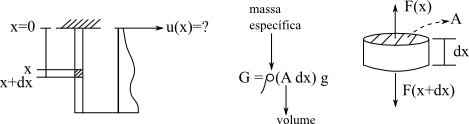
\includegraphics[scale=1.0]{capitulos/capitulo7/figuras/prob_val_cont_barras_placas1.png}
 \caption{Problemas de Valores de Contorno para Barras e Placas}
 \label{fig:prob_val_cont_barras_placas1}
\end{figure}

Alongamento \esp{= \Delta = \displaystyle \frac{du}{dx} \, dx} \\

\esp{F} é proporcional a \esp{\displaystyle \frac{\partial u}{\partial x}\,(x) \Rightarrow F \, (x) = c \, \left. \frac{du}{dx} \, (x) \, \right|_x }

\[
 F\,(x + dx) = c \, \left. \frac{du}{dx} \, \right|_{x + dx}
\]

\begin{eqnarray}
 & \left(
  c \, \displaystyle \frac{du}{dx}
 \right)_{x + \Delta x}
 -
 \left(
  c \, \displaystyle \frac{du}{dx}
 \right)_x
 + G = 0 \nonumber \\
 \nonumber \\
 & \lim_{\Delta x \to 0}
 \displaystyle \frac{
  \left(
   c \, \displaystyle \frac{du}{dx}
  \right)_{x + \Delta x}
  -
  \left(
   c \, \displaystyle \frac{du}{dx}
  \right)_x
 }{\Delta x}
 = -\rho \, A \, g \nonumber \\
 \nonumber \\
 & \displaystyle\frac{d}{dx} \, \left( c \, \frac{du}{dx} \right) = -\rho \, A \, g \nonumber \\
 \nonumber \\
 \label{cap7:sec1:eq1}
 & \mbox{ \framebox{ $ \displaystyle -\frac{d}{dx} \, \left( c \, \frac{du}{dx} \right) = \rho \, A \, g $ } }
\end{eqnarray}

\begin{itemize}

\item Se \esp{c} for constante, a integração é fácil.

\item Se \esp{c = ? \, (u\,(x))}, a integração é não trivial.

\end{itemize}
